% Fig. 1 of the paper as a stand-alone TikZ picture (compile with pdflatex).
% Online: upload to Overleaf as a new project, or paste into any LaTeX editor.
\documentclass[border=4pt]{standalone}
\usepackage{amsmath,amssymb}
\usepackage{tikz}
\usetikzlibrary{positioning,arrows.meta,shapes.geometric,calc,fit}
\begin{document}
% Fig. 1 -- CAD-PSOGSA pipeline (editable copy: CAD-PSOGSA_flowchart.drawio)
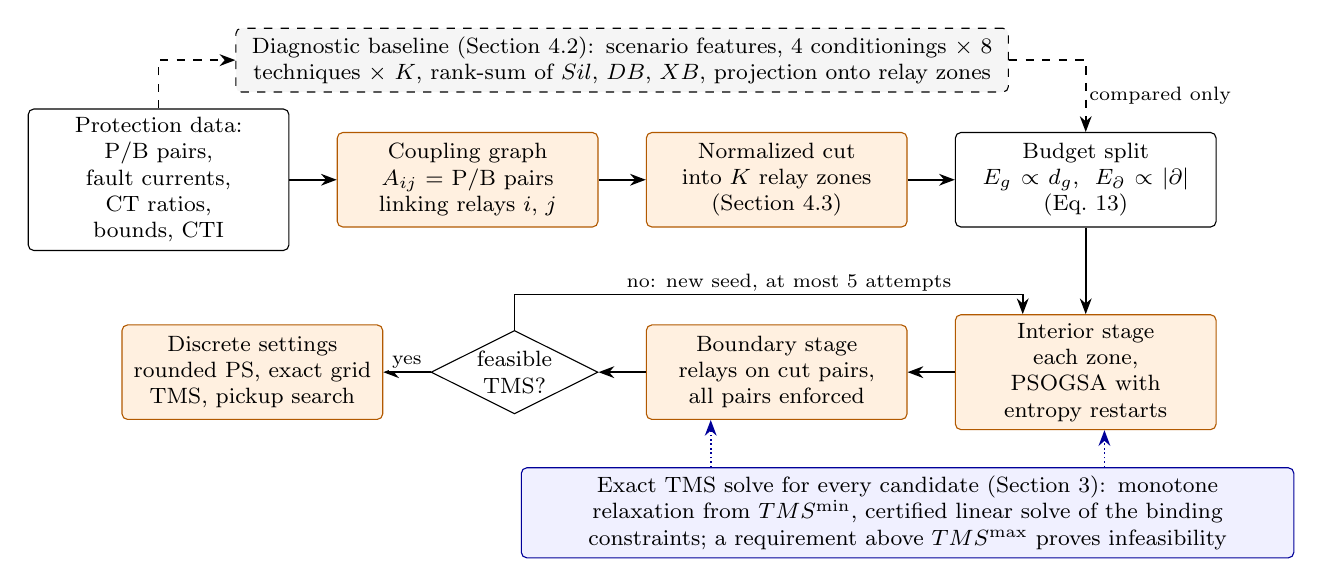
\begin{tikzpicture}[
  font=\footnotesize,
  node distance=4mm and 6mm,
  every node/.append style={execute at begin node={\hyphenpenalty=10000\exhyphenpenalty=10000}},
  blk/.style={draw, rounded corners=2pt, align=center, inner sep=3pt, minimum height=12mm, text width=31mm, fill=white},
  key/.style={blk, fill=orange!12, draw=orange!70!black},
  base/.style={draw, rounded corners=2pt, align=center, inner sep=3pt, dashed, fill=gray!8},
  dec/.style={draw, diamond, aspect=2.0, align=center, inner sep=0.5pt, fill=white},
  arr/.style={-{Stealth[length=2mm]}, semithick},
  lab/.style={font=\scriptsize, fill=white, inner sep=1pt}]
% row 1
\node[blk] (in) {Protection data:\\P/B pairs, fault currents,\\CT ratios, bounds, CTI};
\node[key, right=of in] (graph) {Coupling graph\\$A_{ij}$ = P/B pairs\\linking relays $i$, $j$};
\node[key, right=of graph] (ncut) {Normalized cut\\into $K$ relay zones\\(Section~4.3)};
\node[blk, right=of ncut] (budget) {Budget split\\$E_g \propto d_g$,\ \ $E_\partial \propto |\partial|$\\(Eq.~13)};
% row 2
\node[key, below=11mm of budget] (interior) {Interior stage\\each zone, PSOGSA with\\entropy restarts};
\node[key, left=of interior] (boundary) {Boundary stage\\relays on cut pairs,\\all pairs enforced};
\node[dec, left=of boundary] (feas) {feasible\\TMS?};
\node[key, left=of feas] (disc) {Discrete settings\\rounded PS, exact grid\\TMS, pickup search};
% exact solver used by every fitness evaluation
\node[blk, below=6mm of boundary.south east, anchor=north, text width=96mm, minimum height=9mm, fill=blue!6, draw=blue!60!black] (exact)
  {Exact TMS solve for every candidate (Section~3): monotone relaxation from $TMS^{\min}$,
   certified linear solve of the binding constraints; a requirement above $TMS^{\max}$ proves infeasibility};
% baseline
\node[base, above=5mm of $(graph.north)!0.5!(ncut.north)$, text width=96mm] (valid)
  {Diagnostic baseline (Section~4.2): scenario features, 4 conditionings $\times$ 8 techniques
   $\times$ $K$, rank-sum of $Sil$, $DB$, $XB$, projection onto relay zones};
\draw[arr] (in) -- (graph);
\draw[arr] (graph) -- (ncut);
\draw[arr] (ncut) -- (budget);
\draw[arr] (budget) -- (interior);
\draw[arr] (interior) -- (boundary);
\draw[arr] (boundary) -- (feas);
\draw[arr] (feas) -- node[lab, above]{yes} (disc);
\draw[arr] (feas.north) -- ++(0,4.5mm) -| node[lab, pos=0.27, above]{no: new seed, at most 5 attempts} ([xshift=-8mm]interior.north);
\draw[arr, dashed] (in.north) |- (valid.west);
\draw[arr, dashed] (valid.east) -| node[lab, pos=0.75, right]{compared only} (budget.north);
\draw[arr, densely dotted, blue!60!black] ([xshift=-25mm]exact.north) -- ([xshift=-25mm]exact.north |- boundary.south);
\draw[arr, densely dotted, blue!60!black] ([xshift=25mm]exact.north) -- ([xshift=25mm]exact.north |- interior.south);
\end{tikzpicture}

\end{document}
